\subsection{Counting sort}

\subsubsection{Ý tưởng}
Counting Sort là một thuật toán sắp xếp không dựa trên so sánh, có ưu điểm là tốc độ rất nhanh khi dữ liệu đầu vào thỏa mãn các điều kiện nhất định. Tuy nhiên, thuật toán này có một số hạn chế: chỉ phù hợp với các mảng số nguyên, yêu cầu biết trước khoảng giá trị của các phần tử và tiêu tốn thêm không gian bộ nhớ để tạo mảng đếm.

Có 3 giai đoạn trong thuật toán Counting Sort:
\begin{itemize}
    \item Đếm và phân phối: Tạo một mảng đếm để lưu trữ số lần xuất hiện của mỗi giá trị trong mảng ban đầu. Từ đó, xác định vị trí chính xác của mỗi giá trị trong mảng đã sắp xếp.
    \item Tạo mảng phụ: Tạo một mảng phụ có cùng kích thước với mảng ban đầu. Duyệt mảng ban đầu và đặt từng phần tử vào vị trí chính xác tương ứng trong mảng phụ.
    \item Ghi đè: Ghi đè mảng ban đầu bằng mảng phụ đã sắp xếp.
\end{itemize}


\subsubsection{Các bước hoạt động}
Xét mảng A như sau: 
\begin{center}
   A = \{6, 8, 1, 3, 5, 2\} 
\end{center} 

Bước 1: Xác định giá trị nhỏ nhất và lớn nhất
\[
\text{Min} = 1, \quad \text{Max} = 8
\]

Tạo mảng đếm (\( \text{count} \)) với kích thước \( \text{Max} - \text{Min} + 1 = 8 - 1 + 1 = 8 \):
\[
\text{count} = \{0, 0, 0, 0, 0, 0, 0, 0\}
\]

Bước 2: Đếm số lần xuất hiện của từng phần tử. Duyệt qua mảng \( A \), cập nhật mảng \( \text{count} \):
\[
\begin{aligned}
&\text{A[0] = 6} \quad \Rightarrow \text{count}[6 - 1] = 1 \\
&\text{A[1] = 8} \quad \Rightarrow \text{count}[8 - 1] = 1 \\
&\text{A[2] = 1} \quad \Rightarrow \text{count}[1 - 1] = 1 \\
&\text{A[3] = 3} \quad \Rightarrow \text{count}[3 - 1] = 1 \\
&\text{A[4] = 5} \quad \Rightarrow \text{count}[5 - 1] = 1 \\
&\text{A[5] = 2} \quad \Rightarrow \text{count}[2 - 1] = 1 \\
\end{aligned}
\]

Kết quả:
\[
\text{count} = \{1, 1, 1, 0, 1, 1, 0, 1\}
\]

Bước 3: Tính chỉ số tích lũy trong mảng đếm. Cập nhật \( \text{count} \) thành mảng tích lũy:
\[
\begin{aligned}
\text{count}[1] & = \text{count}[0] + \text{count}[1] = 1 + 1 = 2 \\
\text{count}[2] & = \text{count}[1] + \text{count}[2] = 2 + 1 = 3 \\
\text{count}[3] & = \text{count}[2] + \text{count}[3] = 3 + 0 = 3 \\
\text{count}[4] & = \text{count}[3] + \text{count}[4] = 3 + 1 = 4 \\
\text{count}[5] & = \text{count}[4] + \text{count}[5] = 4 + 1 = 5 \\
\text{count}[6] & = \text{count}[5] + \text{count}[6] = 5 + 0 = 5 \\
\text{count}[7] & = \text{count}[6] + \text{count}[7] = 5 + 1 = 6 \\
\end{aligned}
\]

Kết quả:
\[
\text{count} = \{1, 2, 3, 3, 4, 5, 5, 6\}
\]

Bước 4: Sắp xếp mảng ban đầu vào mảng kết quả. Tạo mảng kết quả \( \text{output} \) với kích thước bằng mảng \( A \). Duyệt ngược qua mảng \( A \) và đặt các phần tử vào đúng vị trí dựa trên mảng \( \text{count} \):
\[
\begin{aligned}
&\text{A[5] = 2} \quad \Rightarrow \text{output}[1] = 2, \quad \text{count}[2 - 1] = 1 \\
&\text{A[4] = 5} \quad \Rightarrow \text{output}[4] = 5, \quad \text{count}[5 - 1] = 4 \\
&\text{A[3] = 3} \quad \Rightarrow \text{output}[2] = 3, \quad \text{count}[3 - 1] = 2 \\
&\text{A[2] = 1} \quad \Rightarrow \text{output}[0] = 1, \quad \text{count}[1 - 1] = 0 \\
&\text{A[1] = 8} \quad \Rightarrow \text{output}[5] = 8, \quad \text{count}[8 - 1] = 5 \\
&\text{A[0] = 6} \quad \Rightarrow \text{output}[3] = 6, \quad \text{count}[6 - 1] = 3 \\
\end{aligned}
\]

Kết quả:
\[
\text{output} = \{1, 2, 3, 5, 6, 8\}
\]

Bước 5: Sao chép mảng \( \text{output} \) vào mảng \( A \).


\begin{figure}[H]
    \centering
    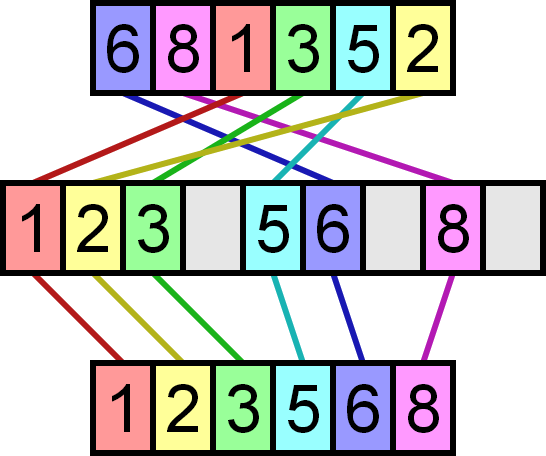
\includegraphics[width=0.8\textwidth]{img/counting-sort.png}
    \caption{\href{https://www.growingwiththeweb.com/images/2014/05/25/counting-sort.svg}{Counting Sort Algorithm Diagram}}
\end{figure}

\subsubsection{Mã giả}
 
\begin{algorithm}[H]
\caption{Counting Sort}
\label{alg:counting-sort}
\begin{algorithmic}

\Require $A$ is an array of size $n$ with integers in the range $0$ to $k$
\Function {counting-sort}{\textit{A}, \textit{k}}
\State Initialize $count[0 \dots k]$ to $0$
\For{$i = 0$ to $n-1$}
    \State $count[A[i]] \gets count[A[i]] + 1$
\EndFor
\For{$i = 1$ to $k$}
    \State $count[i] \gets count[i] + count[i-1]$
\EndFor
\For{$i = n-1$ to $0$}
    \State $B[count[A[i]]-1] \gets A[i]$
    \State $count[A[i]] \gets count[A[i]] - 1$
\EndFor
\State \Return $B$
\EndFunction

\end{algorithmic}
\end{algorithm}


\subsubsection{Độ phức tạp}
\textbf{Độ phức tạp thời gian}


Số phép toán mà thuật toán thực hiện:
\begin{itemize}
    \item Tìm giá trị lớn nhất: Mỗi giá trị phải được đánh giá một lần để tìm ra xem đó có phải là giá trị lớn nhất hay không, do đó cần n phép toán. 
    \item Khởi tạo mảng đếm: Với $k$ là giá trị lớn nhất trong mảng, cần $k + 1$ phần tử trong mảng đếm bao gồm 0. 
    \item Mỗi phần tử trong mảng đếm phải được khởi tạo, do đó cần $k + 1$ phép toán. 
    \item Mỗi giá trị chúng ta muốn sắp xếp được đếm một lần, sau đó xóa, do đó cần 2 phép toán cho mỗi lần đếm, $2n$ phép toán tổng cộng. 
    \item Xây dựng mảng đã sắp xếp: Tạo $n$ phần tử trong mảng đã sắp xếp, cần $n$ phép toán. 

\end{itemize}
Tổng cộng, số phép toán $= n + (k + 1) + 2n + n = 4n + k + 1$. Suy ra độ
phức tạp cho cả ba trường hợp đều là $O(n)$.


\textbf{Độ phức tạp không gian}

Trong quá trình sắp xếp cần 1 mảng đếm và 1 mảng phụ có kích thước bằng kích thước mảng cần sắp xếp, nên độ phức tạp không gian của Counting Sort cũng là $O(n)$.



\subsubsection{Nhận xét}

Sắp xếp đếm (Counting Sort) là một thuật toán sắp xếp rất hiệu quả nhưng có những hạn chế. Nó chỉ có thể được sử dụng khi mảng chỉ chứa các số nguyên và phạm vi giá trị không quá lớn. 


\textbf{Tính ổn định}

Khi đếm số lần xuất hiện của mỗi phần tử, thuật toán duyệt qua mảng từ đầu đến cuối. Các phần tử có cùng giá trị sẽ được đếm liên tiếp nhau. Điều này đảm bảo rằng thứ tự ban đầu của các phần tử giống nhau sẽ được giữ nguyên trong mảng đếm.

Khi xây dựng lại mảng đã sắp xếp, thuật toán duyệt qua mảng đếm từ cuối lên đầu. Đối với mỗi giá trị, nó sẽ lấy ra một số lượng phần tử bằng với số lần đếm tương ứng và đặt chúng vào đúng vị trí trong mảng kết quả. Vì các phần tử giống nhau được đếm liên tiếp nhau trong mảng đếm, nên khi lấy ra và đặt vào mảng kết quả, chúng cũng sẽ được đặt liên tiếp nhau, giữ nguyên thứ tự ban đầu.

Vậy Counting Sort là một thuật toán ổn định.

\textbf{Cải tiến}

Xét mảng $A$ chứa số âm thỏa miền giá trị không quá lớn và ánh xạ $f: x\rightarrow x + min$. Với min, max lần lượt là giá trị nhỏ nhất, lớn nhất của $A$. Do mảng tồn tại số âm nên min < 0, nên $f(A)$ sẽ có giá trị nằm trong khoảng $[0, max - min]$. Lúc này $f(A)$ sẽ thỏa tính chất để có thể thực hiện Counting Sort. Sử dụng tính chất này để sắp xếp cho mảng có số nguyên âm. Và sử dụng ảnh xạ ngược $f^{-1}: x \rightarrow x - min$ để điều chỉnh mảng trở lại mảng ban đầu. 